\section{Evaluation}
\label{sec:eval}

% В данном разделе мы представили результаты апробации трех семантик на нескольких примерах.
In this section we compare the capabilities of a fair conjunction based on structural recursion with a similar approach based on the divergence test of conjuncts~\cite{fair:DivTest}. Also we present the results of the evaluation of three semantics on a set of examples; the semantics were implemented in \textsc{Haskell} in the form of interpreters.

\begin{figure}[h!]
\centering
\begin{tabular}{c}
\begin{lstlisting}
let rec add$^o$ x y xy =
  (x === Zero /\ y === xy) \/
  fresh (x') (
    x === Succ x' /\ 
    add$^o$ x' (Succ y) xy)
\end{lstlisting}
\end{tabular}
\caption{Relational addition of Peano numbers}
\label{fair:lst-addo}
\end{figure}

The approach based on the divergence test has similar to our behavior. When evaluating a conjunct before unfolding, we compute the predicate. And depending on the result, we either perform
the unfolding or begin to evaluate another conjunct. However, this approach has two key differences.

First, it uses a different predicate that detects a divergence. The predicate is as follows: if a call in the current conjunct is more general than one of the enclosing ones to the same relation, it
is necessary to evaluate another conjunct. Both predicates are not always efficient. Our predicate based on structural recursion is obviously not efficient in relations without structural recursion.
In this case, a naive fair conjunction will be used. At the same time, the predicate based on the divergence test is also not efficient for some programs. For example,
a query \lstinline{add$^o$ q Zero Zero} of relation \lstinline{add$^o$} (Fig.~\ref{fair:lst-addo}) diverges but no one of the calls in the sequence of evaluation

\begin{lstlisting}
add$^o$ q   Zero               Zero, 
add$^o$ q$_1$ (Succ Zero)          Zero, 
add$^o$ q$_2$ (Succ (Succ Zero)) Zero, 
...
\end{lstlisting}

is more general than its predecessors. As a result, the conjunction \linebreak \lstinline{(add$^o$ q Zero Zero /\ q === Zero)} will give a correct answer and diverge. At the same time,
the relation \lstinline{add$^o$} is structurally recursive in the first argument and this argument is fresh. Therefore, our approach will evaluate the second conjunct and then
the first conjunct will converge.

Second, the approach based on the divergence test moves to another conjunct in a different way. When we want to evaluate a conjunction \lstinline{(A /\ B)} we evaluate the first
conjunct \lstinline{A}. If after some steps we get \lstinline{A$'$} which diverges, we change the order in the original conjunction and begin to evaluate \lstinline{(B /\ A)}.
In other words, we are looking for a converging conjunct to be evaluated first. This behavior selects the optimal order of the conjuncts, but is not applicable in the case when
all the conjuncts diverge, being evaluated in isolation. Thus, the query \lstinline{divergence$^o$ l} (see Fig.~\ref{fair:lst-repeato}) will detect divergence in both conjuncts,
then will stop and report the impossibility to continue the evaluation. At the same time our approach allows to find the answer and prove the absence of other answers.

To summarize, our approach and the approach based on the divergence test may be inefficient on some examples, and our approach saves more information when moving to another conjunct,
which allows us to correctly evaluate some diverging programs.

\begin{figure}
\centering
\begin{minipage}{.5\textwidth}
  \centering
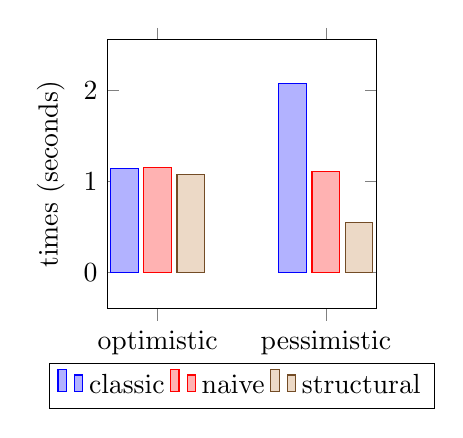
\begin{tikzpicture}
\begin{axis}[
    ybar, ymax = 2, ymin = 0.15,
    enlargelimits=0.3,
    width=5cm, height=5cm,
    legend style={at={(0.5,-0.2)},
      anchor=north,legend columns=-1},
    ylabel={times (seconds)},
    symbolic x coords={optimistic, pessimistic},
    xtick=data
    ]
\addplot coordinates {(optimistic,1.142) (pessimistic,2.073)};
\addplot coordinates {(optimistic,1.151) (pessimistic,1.110)};
\addplot coordinates {(optimistic,1.077) (pessimistic,0.542)};
\legend{classic,naive,structural}
\end{axis}
\end{tikzpicture}
  \captionof{figure}{revers$^o$ forward evaluation \\ for a list with a length of 90}
  \label{fair:plot-reverso}
\end{minipage}%
\begin{minipage}{.5\textwidth}
  \centering
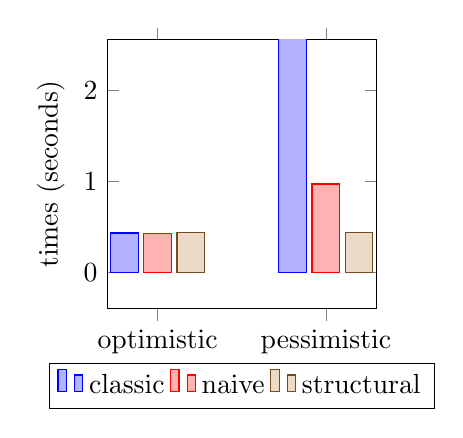
\begin{tikzpicture}
\begin{axis}[
    ybar, ymax = 2, ymin = 0.15,
    enlargelimits=0.3,
    width=5cm, height=5cm,
    legend style={at={(0.5,-0.2)},
      anchor=north,legend columns=-1},
    ylabel={times (seconds)},
    symbolic x coords={optimistic, pessimistic},
    xtick=data
    ]
\addplot coordinates {(optimistic,0.430) (pessimistic,300)};
\addplot coordinates {(optimistic,0.428) (pessimistic,0.969)};
\addplot coordinates {(optimistic,0.433) (pessimistic,0.432)};
\legend{classic,naive,structural}
\end{axis}
\end{tikzpicture}
 \captionof{figure}{sort$^o$ forward evaluation \\ for a list with a length of 5}
\label{fair:plot-sorto}
\end{minipage}
\end{figure}

\begin{figure}
\centering
\begin{minipage}{.5\textwidth}
  \centering
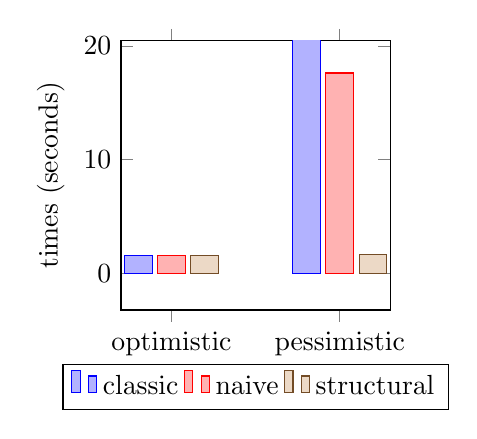
\begin{tikzpicture}
\begin{axis}[
    ybar, ymax = 16, ymin = 1.2,
    enlargelimits=0.3,
    width=5cm, height=5cm,
    legend style={at={(0.5,-0.2)},
      anchor=north,legend columns=-1},
    ylabel={times (seconds)},
    symbolic x coords={optimistic, pessimistic},
    xtick=data
    ]
\addplot coordinates {(optimistic,1.574) (pessimistic,300)};
\addplot coordinates {(optimistic,1.579) (pessimistic,17.604)};
\addplot coordinates {(optimistic,1.585) (pessimistic,1.646)};
\legend{classic,naive,structural}
\end{axis}
\end{tikzpicture}
 \captionof{figure}{``The Tower of Hanoi'' \\ solver evaluation}
\label{fair:plot-hanoi}
\end{minipage}%
\begin{minipage}{.5\textwidth}
  \centering
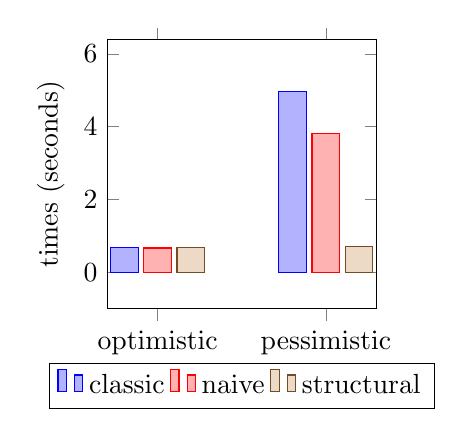
\begin{tikzpicture}
\begin{axis}[
    ybar, ymax = 5, ymin = 0.375,
    enlargelimits=0.3,
    width=5cm, height=5cm,
    legend style={at={(0.5,-0.2)},
      anchor=north,legend columns=-1},
    ylabel={times (seconds)},
    symbolic x coords={optimistic, pessimistic},
    xtick=data
    ]
\addplot coordinates {(optimistic,0.669) (pessimistic,4.956)};
\addplot coordinates {(optimistic,0.663) (pessimistic,3.820)};
\addplot coordinates {(optimistic,0.675) (pessimistic,0.712)};
\legend{classic,naive,structural}
\end{axis}
\end{tikzpicture}
 \captionof{figure}{``Bridge and torch problem'' \\ solver evaluation}
\label{fair:plot-bridge}
\end{minipage}
\end{figure}

Now we will discuss evaluation. For evaluation we've chosen two simple programs (list reversing and list sorting) and three more complicated (the ``Hanoi Towers''\footnote{\url{https://en.wikipedia.org/wiki/Tower_of_Hanoi}} solver, the
``Bridge and torch problem''\footnote{\url{https://en.wikipedia.org/wiki/Bridge_and_torch_problem}} solver and ``Water pouring puzzle''\footnote{\url{https://en.wikipedia.org/wiki/Water_pouring_puzzle}} solver).
% Для каждой программы мы сделали две версии. Оптимистичная версия --- это программа, в которой мы вручную подобрали оптимальный порядок конъюнктов и пессиместичная версия --- программа с неоптимальным порядком конъюнктов. В последующих диаграммах и таблице указаны средние значения 10 запусков тестов. Также для наивной равномерной конъюнкции мы подобрали количество разверток вручную. Для равномерной конъюнкции, основанной на структурной рекурсии, N было фиксировано и равно 100.
Each program was written in two versions: ``optimistic'' (with the order of important conjuncts set to provide the best performance) and ``pessimistic'' (with the order of important
conjuncts set to provide the worst performance). Also we evaluated list reversing and list sorting in both directions. In the case of the list reversing, queries \lstinline{(revers$^o$ [1;2;3] q)} and \lstinline{(revers$^o$ q [1;2;3])}\! will give the same answer \lstinline{q = [3;2;1]} but the ``optimistic'' order of conjuncts is different for them. In the case of list sorting, queries \lstinline{(sort$^o$ [1;2;3] q)} and \lstinline{(sort$^o$ q [1;2;3])} will give different answers. The first one gives sorted list \lstinline{q = [1;2;3]}, the second one gives all permutations of list \lstinline{[1;2;3]}\!\!. 

All benchmarks were run ten times, and the average time was taken. For the naive fair conjunction we cherry-picked the best value of unfolding bound manually. For the fair conjunction
based on structural recursion the bound was set to 100, structural arguments for each relations were detected automatically.

% На изображениях 12-15 представлены результаты апробации в виде столбцовых диаграмм. В оптимистичном случае результаты схожи для всех семантик. В пессиместичном случае время работы напрпавленной конъюнкции резко возрастает, время работы наивной равномерной конъюнкции также ворзрастает, но не так сильно. Равномерная конъюнкция, основанная на структурной рекурсии, демострирует схожую эффективность в сравнении с оптимистичным случаем.
Fig.~\ref{fair:plot-reverso}-\ref{fair:plot-bridge} show the results of evaluation in the form of bar charts. In the optimistic case, the results are similar for all semantics.
In the pessimistic case the evaluation time of the directed conjunction rapidly increases, the evaluation time of the naive fair conjunction also increases, but not so much.
The fair conjunction based on structural recursion demonstrates a similar efficiency as in the optimistic case.

\begin{figure}[h!]
  \small
  \centering
  \begin{tabular}{ c | c | c | c | c | c | c | c }
    \multirow{2}{*}{relation} & \multirow{2}{*}{size} & 
    \multicolumn{2}{c}{directed conjunction} &
    \multicolumn{2}{c}{naive fair conjunction} &
    \multicolumn{2}{c}{structural recursion} \\
    \cline{3-8}
    & & optimistic & pessimistic & optimistic & pessimistic & optimistic & pessimistic  \\ 
    \hline
    \multirow{3}{*}{\begin{tabular}{c} forward \\ revers$^o$ \end{tabular}}
                 & 30   & 0.465 & 0.532  & 0.468 & 0.461   & 0.438 & 0.425 \\
                 & 60   & 0.579 & 0.828  & 0.577 & 0.658   & 0.545 & 0.450 \\
                 & 90   & 1.142 & 2.073  & 1.151 & 1.110   & 1.077 & 0.542 \\
    \hline
    \multirow{3}{*}{\begin{tabular}{c} backward \\ revers$^o$ \end{tabular}}
                 & 30   & 0.541 & 0.573  & 0.550 & 0.540  & 0.516 & 0.518 \\
                 & 60   & 0.637 & 0.867  & 0.642 & 0.805  & 0.636 & 0.637 \\
                 & 90   & 1.268 & 1.778  & 1.274 & 1.359  & 1.289 & 1.273 \\
    \hline
    \multirow{5}{*}{\begin{tabular}{c} forward \\ sort$^o$ \end{tabular}}
                 & 3    & 0.418 & 0.432  & 0.420 & 0.420  & 0.424 & 0.425 \\
                 & 4    & 0.424 & 3.924  & 0.424 & 0.455  & 0.429 & 0.429 \\
                 & 5    & 0.430 & $>$300 & 0.428 & 0.969  & 0.433 & 0.432 \\
                 & 6    & 0.434 & $>$300 & 0.430 & 11.577 & 0.434 & 0.437 \\
                 & 30   & 1.664 & $>$300 & 1.636 & $>$300 & 1.723 & 1.751 \\ 
    \hline
    \multirow{4}{*}{\begin{tabular}{c} backward \\ sort$^o$ \end{tabular}}
                 & 3    & 0.511 &  0.511 & 0.509 & 0.513  & 0.516 & 0.518 \\
                 & 4    & 0.525 &  0.823 & 0.534 & 0.539  & 0.534 & 0.530 \\
                 & 5    & 0.667 & 69.725 & 0.692 & 1.443  & 0.689 & 0.697 \\
                 & 6    & 2.880 & $>$300 & 2.891 & 56.107 & 2.921 & 2.936 \\
    \hline
    hanoi$^o$    & -    & 1.574 & $>$300 & 1.579 & 17.604 & 1.585 & 1.646 \\
    \hline
    bridge$^o$   & -    & 0.669 & 4.956  & 0.663 & 3.820  & 0.675 & 0.712 \\
    \hline
    water$^o$    & -    & 3.132 & $>$300 & 3.168 & $>$300 & 3.220 & 3.414

  \end{tabular}
  \caption{The results of evaluation: running times of benchmarks in seconds}
  \label{fair:evaluation-table}
\end{figure}

% Более подробно результаты представлены на изображении 16. Можно заметить, что время работы программы sorto в пессиместичном случае очень быстро растет с увеличением длины списка для направленной конъюнкции и наивной равномерной. В случае с равномерной конъюнкцией, основанной на структурной рекурсии, пессиместичный случай растет сопостовимо с оптимистичным.
The results are presented in more detail in Fig.~\ref{fair:evaluation-table}. ``Hanoi Towers'' solver has name \lstinline{hanoi$^o$}, ``Bridge and torch problem'' solver has name \lstinline{bridge$^o$} and ``Water pouring puzzle'' solver has name \lstinline{water$^o$}. We can conclude that forward and backward \lstinline{sort$^o$} runtime in the pessimistic case increases very rapidly with increasing the list length for directed and naive fair conjunctions. In the case of the fair conjunction based on structural recursion the running time in pessimistic case increases on a par with that in the optimistic one. Also  the solver \lstinline{water$^o$} very slow in the pessimistic case for directed and naive fair. However, fair conjunction based on structural recursion pessimistic case is no different from an optimistic case.


% Подводя итог, равномерная конъюнкция, основанная на структурной рекурсии сопоставима по эффективности с направленной конъюнкцией. Более того, это конъюнкция слабо зависит от порядка конъюнктов.
To summarize, the fair conjunction based on structural recursion does not introduce any essential overhead in comparison with directed conjunction in an optimistic case. At the same time it
weakly depends on the order of the conjuncts, and thus demonstrates much better performance in the pessimistic case.
